\newcommand{\tpar}[1]{ \multicolumn{5}{p{\textwidth}}{#1} \vspace{0.5em}}
\newcommand{\tparx}[1]{ \multicolumn{4}{p{\textwidth}}{#1} \vspace{0.5em}}


\begin{longtable}[h]{L{0.5cm} L{0.8cm} L{4.0cm} L{4.0cm} L{5.0cm}}
&Use cases &
Original text &
English translation &
Comments \\*
\hline \\*
\endhead
\tpar{ 
\textbf{Overbygning}: 530 Prosjektering, Kap. 8 Helsveist spor, 2.1.
} \\*
&\#4 &
De store krefter som kan forekomme i et helsveist spor stiller strenge krav til sporets konstruksjon. &
The large forces that may occur in a welded track makes stringent demands on the track construction.& 
This sentence is not normative, and is unlikely to have any use in automated verification.
\\
& & & & \\
\tpar{ 
\textbf{Overbygning}: 530 Prosjektering, Kap. 8 Helsveist spor, 2.1.3 a)
} \\*
&\#4 &
Ballasten skal på linjen og i hovedspor på statsjoner være fullverdig grovpukk (av størrelse 31.5 -- 63 mm) &
The ballast on the line and in the main track at stations must be purely coarse crushed stone  (size from 31.5 to 63 mm) &
This is a specification which is absolute, and rules out 
the need for specifying this as a part of the design, because
it is not part of a specific station.
It can still be valuable to support this sentence in a CNL, 
and in a formal representation.
\\
& & & & \\
\tpar{ 
\textbf{Overbygning}: 530 Prosjektering, Kap. 8 Helsveist spor, 2.1.2 a)
}\vspace{0.5em} \\* 
&\#1 &
Minste kurveradius for helsveist med betongsviller skal være 250 m. &
The lowest allowable radius of curvature for whole welded track on concrete sleepers is 250 m.& 
{This is a typical example of static infrastructure verification, expressible in Datalog as: \newline	
\footnotesize{
error(Segment) :- trackSegment(Segment), trackSegmentRadius(Segment, Radius), Radius < 250.
}
}
\\
& & & & \\
\tpar{ 
\textbf{Signal}: 550 Prosjektering, Kap. 6 Lyssignal, 2.1.2 j)
}\vspace{0.5em} \\* 
&\#1 &
Et innkjørhovedsignal skal plasseres $\geq$ 200 meter foran innkjørtogveiens første sentralstilte, motrettede sporveksel, se Figur 5. 
&
A home main signal shall be placed at least 200 m in front of the first controlled, facing switch in the entry train path (see Figure 5).
& 
{This is the example that we have been using most frequently for the RailCons verification tool. Datalog:\newline
\footnotesize{
error(Sig,Sw) :- firstFacing(Bdry, Sw, Dir), homeSignalBetween(Sig, Bdry, Sw), distance(Sig, Sw, Dir, L), L < 200.
}
}
\\
& & & & \\

\tpar{ 
\textbf{Signal}: 550 Signal, Kap. 5 Forriglingsutrustning, 2.8.1 Dekningsgivende objekt
}\vspace{0.5em} \\* 
&\#1, \#2 &
Følgende objekt kan være dekningsgivende: Hovedsignal, Dvergsignal, Sporveksel, Sporsperre, Avsporingstunge, Signal E35 Stoppskilt.
Et hovedsignal skal vise signal ”Stopp” for å være dekningsgivende.
&
The following objects can provide flank protection: main signal, shunting signal, switch, derailer, derailing tongue, signal E35 stop sign.
A main signal must display "stop" to provide flank protection.
&
This regulation is relevant both for \textbf{specifying} the control system, and for verifying the \textbf{implementation}. The specification chooses which objects to use for flank protection (\textbf{static}) and what state they can be used in, while the implementation must correctly enforce the conditions saying which message the signal displays (\textbf{dynamic}).
\\
& & & & \\
\tpar{ 
\textbf{Signal}: 550 Prosjektering, Kap. 6 Lyssignal, 2.1.2 i)
}\vspace{0.5em} \\* 
&\#1, \#3 &
Et hovedsignal bør ikke plasseres i tunneler, på bruer, eller andre steder hvor en eventuell togstans og dermed muligheten for avstigning, vil medføre fare. 
&
A main signal should not be placed in tunnels, on bridges, or other places where halting trains and thus the possibility of disembarking, can impose dangers.
& 
Here we have an example of a ``\emph{should}'' modality, where the 
static infrastructure verification could issue a warning, but not an error. 
Also, it could be required to document the alternatives that were considered
when deciding on the design.
\\
& & & & \\
\tpar{ 
\textbf{Signal}: 550 Prosjektering, Kap. 5 Forriglingsutrustning, 4.1.1.1 i)
}\vspace{0.5em} \\* 
&\#2 &
For at en togvei skal kunne fastlegges, skal et objekt som gir dekning til togveien være dekningsgivende. 
&
For a train route to be deactivated, any object giving flank protection must be in a protecting state.
& 
This regulation concerns only the state of the control system, and as such 
relates to the implementation of the control system and not the static infrastructure specification.
\\
& & & & \\ 
& & & & \\ 
& & & & \\ 
\tpar{ 
\textbf{Overbygning}: 530 Prosjektering, Kap. 5 Sporets trasé, 3.1 Dimensjonerende parametre
} \\*
& \#1 & 
See table below.
& (a) minimum radius, (b) maximal superelevation, 
(c) limit on superelevation cause by derailment risk at low speeds,
(d) limit for superelevation rate of change,
(e) limit for superelevation deficit.
&
Limiting values are organized in a table for use in formulas in other sections.
\\*
&\tparx{
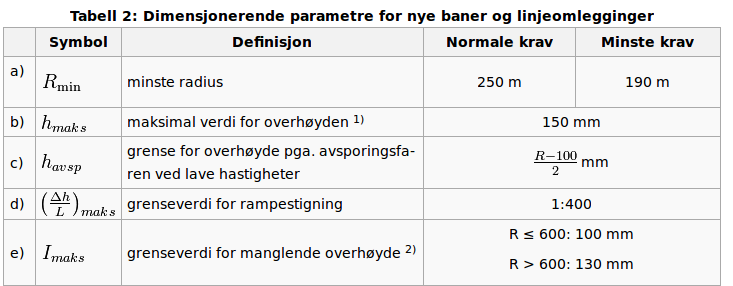
\includegraphics[width=0.9\textwidth]{tabless.png}
} 
\\
& & & & \\
\tpar{ 
\textbf{Overbygning}: 530 Prosjektering, Kap. 5 Sporets trasé, 3.7 Sporveksler og sporforbindelser
} \\*
& \#1 & 
Avstanden mellom sporveksel og overgangskurve, sirkelkurve, bru eller annen motstående sporveksel skal ikke være mindre enn avstanden M gitt i \emph{Kurver uten overgangskurver}, krav b). M skal imidlertid ikke være kortere enn 6 m. 
& 
The distance between the switch point and the transition curve, circle curve, bridge or other opposite switch point should not be less than the distance M given in section \emph{``curves without transition curves''}, requirements b). M shall not be shorter than 6 m.
&
The parameter $M$ is explained by the figure below. Reference is given to 
another section of the regulations.
\\*
&\tparx{
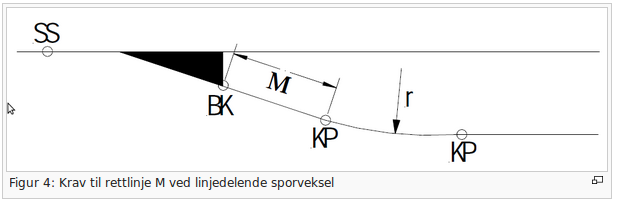
\includegraphics[width=0.8\textwidth]{figuress.png}} \\
& & & & \\
\tpar{ 
\textbf{Overbygning}: 530 Prosjektering, Kap. 5 Sporets trasé, 5 Største hastighet -- sporets geometri
} \\*
& \#1 & 
Hastigheten i en kurve skal ikke være større enn:
{\footnotesize
\begin{equation*}
V = 0,291 \cdot\sqrt{R\left(h +I_{\text{maks}}\right)}\quad \text{(5)}
\end{equation*}
}
Hvis ligning 5 i tilfeller med falsk overhøyde gir lavere verdi enn 20 km/h gjelder $V = 20$ km/h.
&
The speed in a curve shall not exceed:
{\footnotesize
\begin{equation*}
V = 0,291 \cdot\sqrt{R\left(h +I_{\text{maks}}\right)}\quad \text{(5)}
\end{equation*}
}
If Eq. 5 gives a lower value than 20 km/h in situations with false superelevation, then $V = 20$ km/h shall be used.
& 
Use of equations with designed and given parameters.\\
& & & & \\
\tpar{ 
\textbf{Signal}: 552 Vedlikehold, Kap. 6 Lyssignal, 3 Lyssignaler
} \\*
& \#3, \#4 & 
Dersom lyssignal er vridd eller på annen måte kommet ut av stilling skal dette utbedres snarest. 
&
If a signal is twisted or in other ways are out of position, this shall be fixed as soon as possible.
& 
Typical maintenance regulation. Here, it might be sufficient to identify this as a \emph{checklist item}, for 
maintenance scheduling and reporting purposes.
\end{longtable}
